\chapter{Vorstellung ausgewählter Szenarien} \label{chap:Vorstellung_Szenarien}
\thispagestyle{empty}
Um geeignete Szenarien für die Simulation zu erstellen, wurden verschiedene Quellen berücksichtigt:
\begin{itemize}
    \item betriebsinterne Szenariendatenbank
    \item Normen und Richtlinien 
    \item eigene Überlegungen nach Systemanalyse
\end{itemize}
Es steht intern eine Szenariendatenbank zur Verfügung. Für diese Simulation sind viele Szenarien allerdings nicht von Relevanz, da die Pfadplanung von einem übergeordneten Modul realisiert wird und bspw. Kreuzungsszenarien zu Kurvenszenarien reduziert werden. In \cite{ISO15622} und \cite{NCAP2024} werden verschiedene Szenarien für die Einhaltung gesetzlicher Vorschriften und ACC Systeme definiert. Weiterhin wurden auch Negativtests implementiert. Dabei wird ein Szenario bewusst so parametriert, dass es der Simulation nicht möglich ist die KPIs einzuhalten. In diesen Fällen ist ein fehlschlagen eines Test als positiv zu werten. Ein Test schlägt fehl, wenn die Grenzwerte nicht überschritten wurden sind.\medskip

\noindent Im folgenden werden exemplarisch einzelne Szenarien näher erläutert. 

\section{Szenario: Gerade mit initialem Versatz} \label{sec:straight_offset}
Das Ego startet auf einer Geraden. Die Initialgeschwindigkeit ist gleich der Pfadgeschwindigkeit. Es besteht ein initialer lateraler Versatz von der Ego Position zum gewünschten Pfad. Das Ego sollte den initialen Versatz abbauen und mit der Pfadgeschwindigkeit auf dem gewünschten Pfad fahren. Die gerine Komplexität und Parameteranzahl des Szenarios ermöglichen eine einfache Analyse von Auswirkungen der Veränderung eines Parameters bei gleichzeitiger Konstanthaltung der anderen Parameter. Dafür wurde in allen Diagrammen das gleiche MPC-Parameterset und das gleiche Fahrzeug verwendet.
\begin{figure}[ht]
    \centering
    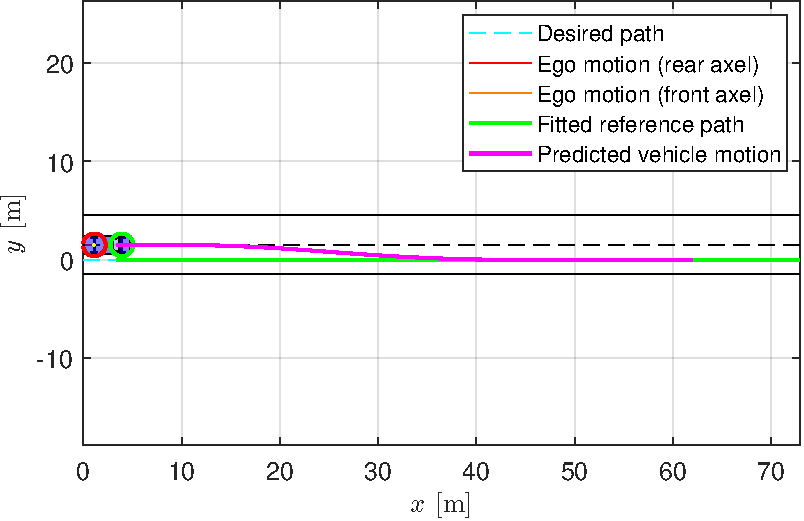
\includegraphics[width=0.5\textwidth]{figures/3_Implementierung/Straight_Offset/test_straight_depiction.pdf}
    \caption{Darstellung des Szenarios: Gerade mit initialem Versatz}
    \label{fig:test_straight_depiction}
\end{figure}

\subsection{Parametrierung}
Die Parameter für dieses Szenario sind:
\begin{itemize}
    \item Versatz $[m]$: $s_{offset} \in [-1.5,1.5]$ 
    \item Initialgeschwindigkeit $[km\cdot h^{-1}]$: $v_{Ego} \in [10,v_{vehicle,max}]$
    \item verwendetes MPC Parameterset 
\end{itemize}

\subsection{Abgetestete KPIs}
Es wurden Test für folgende KPIs mit den dazugehörigen Grenzwerten implementiert:

\medskip\noindent\textbf{Einschwingzeit:}: der laterale Versatz sollte innerhalb einer bestimmten Zeit abgebaut werden: $t_{settle} < kpi_{t_{settle}}$

\noindent Eine Variation des Versatzes bei gleicher Geschwindigkeit von 50 km/h (Abbildung \ref{fig:varOffset_50kmh_s-Error}) führt zu sehr ähnlichem Verhalten und einer nahezu identischen Reaktionszeit (erster Nulldurchlauf). Je größer der Versatz desto höher ist das Überschwingen auf der anderen Seite des Pfades, was zu einer längeren Einschwingzeit führt. Bei der Variation der Geschwindigkeit (Abbilfung \ref{fig:varVelo_1mOffset_s-Error}) und konstantem Versatz von 1 m verschiebt sich der Zeitpunkt des maximalen Überschwingens nach hinten, je geringer die Geschwindigkeit wird.  Durch die Wahl eines Grenzwertes der maximalen Pfadabweichung kann die Einschwingzeit bestimmt werden, indem das letzte Überschreiten des Grenzwertes ermittelt wird.
\begin{figure}[ht]
    \centering
    \begin{subfigure}[b]{.49\textwidth}
        \centering
        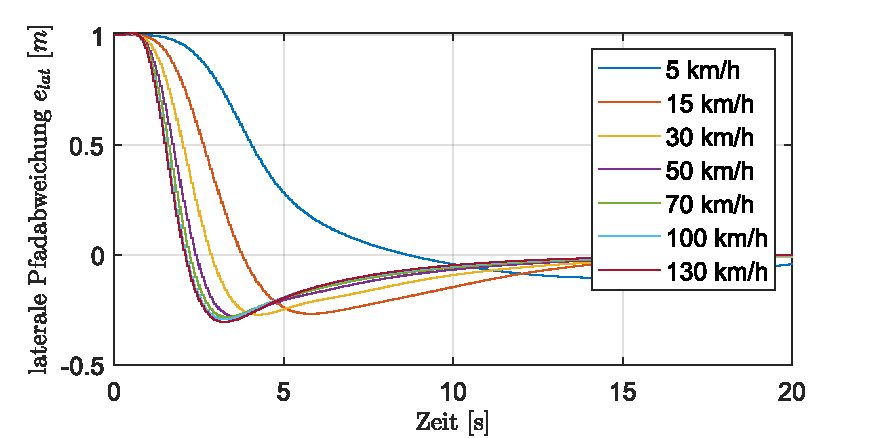
\includegraphics[width=\textwidth]{figures/3_Implementierung/Straight_Offset/varVelo_1mOffset_s-Error.pdf}
        \caption{Variation der Initialgeschwindigkeit}
        \label{fig:varVelo_1mOffset_s-Error}
    \end{subfigure}
    \hfill
    \begin{subfigure}[b]{.49\textwidth}
        \centering
        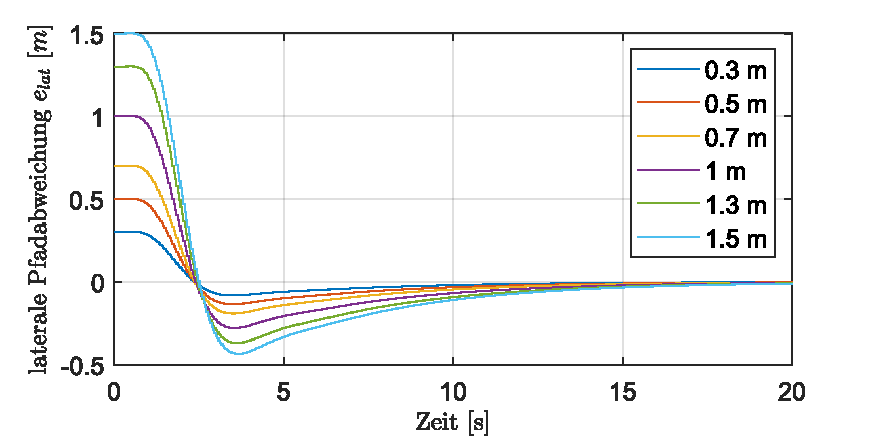
\includegraphics[width=\textwidth]{figures/3_Implementierung/Straight_Offset/varOffset_50kmh_s-Error.pdf}
        \caption{Variation des initialen Versatzes}
        \label{fig:varOffset_50kmh_s-Error}
    \end{subfigure}
    \caption{KPI Pfadabweichung abhängig der Simulationsparameter}
    \label{fig:Straight_Offset_s-Error}
\end{figure}

\medskip\noindent\textbf{longitudinale Geschwindigkeit:} die Geschwindigkeitsabweichung zum Pfad darf den Grenzwert nicht überschreiten: $|v_{Long} - v_{Path}| < kpi_{v_{diff}}$

\noindent Die Pfadgeschwindigkeit ist in der Implementierung der MPFC ein Optimierungsparameter. Ein verhindern des Überschreitens der Pfadgeschwindigkeit ist nicht garantiert. Um den Versatz möglichst schnell abzubauen beschleunigt der Regler das Fahrzeug. Dies ist vorallem bei niedrigeren Geschwindigkeiten und höheren Versätzen zu beobachten, siehe Abbildungen \ref{fig:Straight_Offset_s-Error}.   
\begin{figure}[ht]
    \centering
    \begin{subfigure}[b]{.49\textwidth}
        \centering
        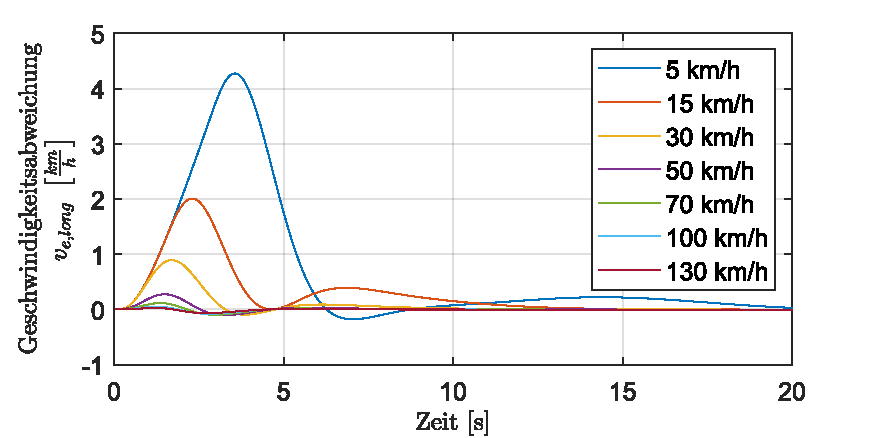
\includegraphics[width=\textwidth]{figures/3_Implementierung/Straight_Offset/varVelo_1mOffset_v-Diff.pdf}
        \caption{Variation der Initialgeschwindigkeit}
        \label{fig:varVelo_1mOffset_v-Diff}
    \end{subfigure}
    \hfill
    \begin{subfigure}[b]{.49\textwidth}
        \centering
        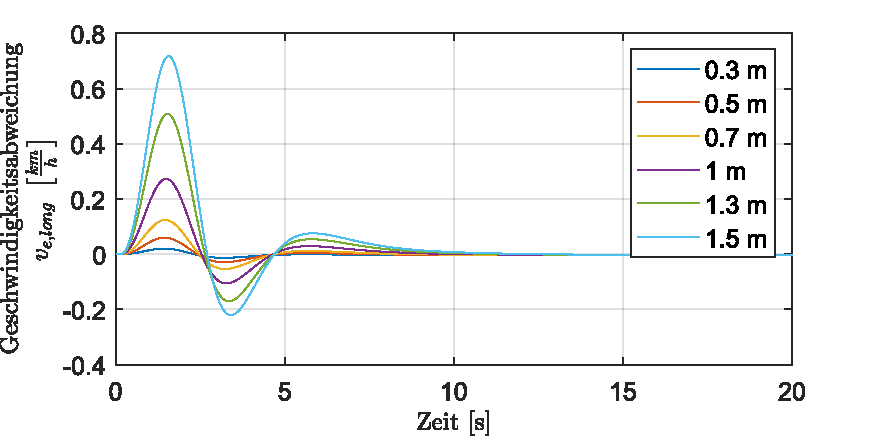
\includegraphics[width=\textwidth]{figures/3_Implementierung/Straight_Offset/varOffset_50kmh_v-Diff.pdf}
        \caption{Variation des initialen Versatzes}
        \label{fig:varOffset_50kmh_v-Diff}
    \end{subfigure}
    \caption{KPI Geschwindigkeitsabweichung abhängig der Simulationsparameter}
    \label{fig:Straight_Offset_v-Diff}
\end{figure}

\medskip\noindent\textbf{laterale Beschleunigung:} der gleitende Mittelwert über eine halbe Sekunde darf den Grenzwert nicht überschreiten: $a_{Lat} < kpi_{a_{Lat}}$

\noindent Wie aus Abbildung \ref{fig:Straight_Offset_a-Lat} hervorgeht führen höhere Geschwindigkeiten und ein größerer initialer Versatz erwartungsgemäß zu größeren Amplituden.
\begin{figure}[ht]
    \centering
    \begin{subfigure}[b]{.49\textwidth}
        \centering
        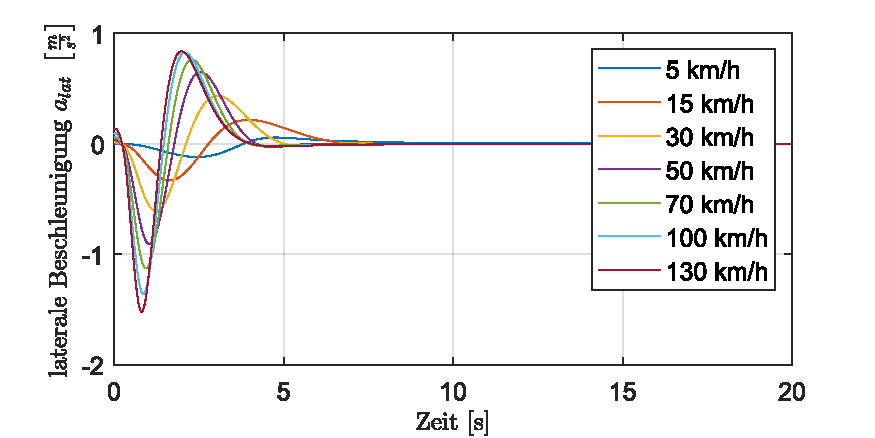
\includegraphics[width=\textwidth]{figures/3_Implementierung/Straight_Offset/varVelo_1mOffset_a-Lat.pdf}
        \caption{Variation der Initialgeschwindigkeit}
        \label{fig:varVelo_1mOffset_a-Lat}
    \end{subfigure}
    \hfill
    \begin{subfigure}[b]{.49\textwidth}
        \centering
        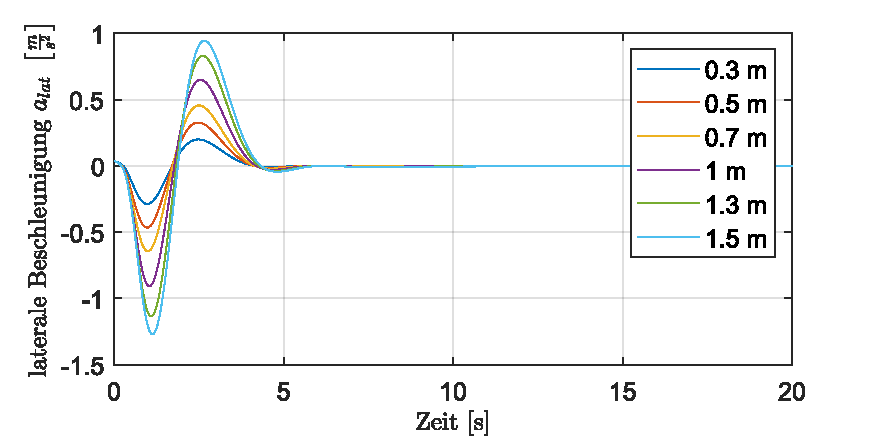
\includegraphics[width=\textwidth]{figures/3_Implementierung/Straight_Offset/varOffset_50kmh_a-Lat.pdf}
        \caption{Variation des initialen Versatzes}
        \label{fig:varOffset_50kmh_a-Lat}
    \end{subfigure}
    \caption{KPI laterale Beschleunigung abhängig der Simulationsparameter}
    \label{fig:Straight_Offset_a-Lat}
\end{figure}

\medskip\noindent\textbf{lateraler Ruck:} der Gleitende Mittelwert über eine halbe Sekunde darf den Grenzwert nicht überschreiten: $j_{Lat} < kpi_{j_{Lat}}$

\noindent Wie aus Abbildung \ref{fig:Straight_Offset_j-Lat} hervorgeht führen höhere Geschwindigkeiten und ein größerer initialer Versatz erwartungsgemäß zu größeren Amplituden.
\begin{figure}[ht]
    \centering
    \begin{subfigure}[b]{.49\textwidth}
        \centering
        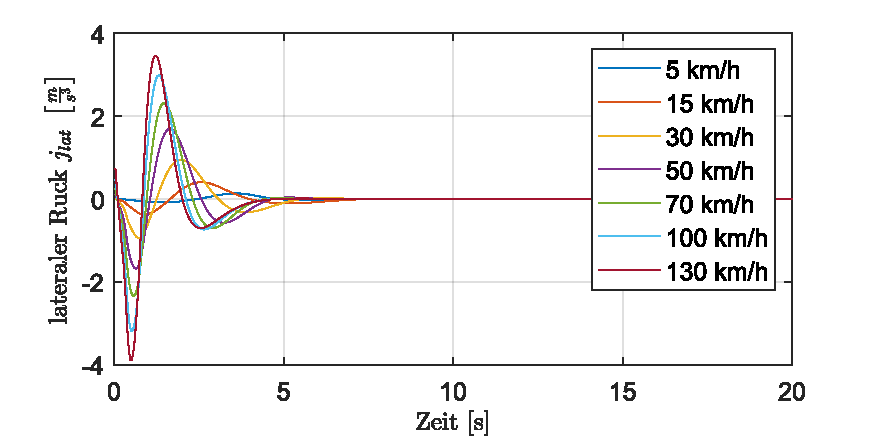
\includegraphics[width=\textwidth]{figures/3_Implementierung/Straight_Offset/varVelo_1mOffset_j-Lat.pdf}
        \caption{Variation der Initialgeschwindigkeit}
        \label{fig:varVelo_1mOffset_j-Lat}
    \end{subfigure}
    \hfill
    \begin{subfigure}[b]{.49\textwidth}
        \centering
        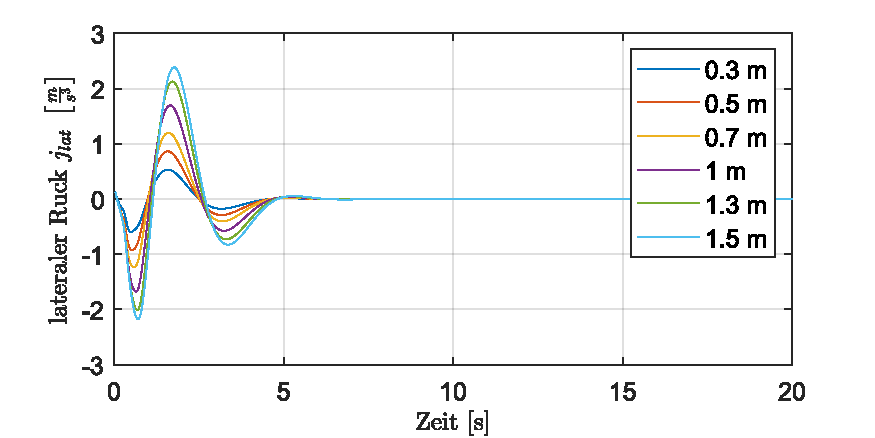
\includegraphics[width=\textwidth]{figures/3_Implementierung/Straight_Offset/varOffset_50kmh_j-Lat.pdf}
        \caption{Variation des initialen Versatzes}
        \label{fig:varOffset_50kmh_j-Lat}
    \end{subfigure}
    \caption{KPI lateraler Ruck abhängig der Simulationsparameter}
    \label{fig:Straight_Offset_j-Lat}
\end{figure}

\section{Szenario: Kurve negativ} \label{sec:kurveNegativ}
Das Ego startet mit einer Initialgeschwindigkeit, welche der Pfadgeschwindigkeit entspricht auf einer Geraden. An die Gerade schließt sich eine Kurve an, welche in einen Kreis endet. Der Radius des Kreises ist kleiner als der minimale Wendekreis des Fahrzeugs. Das Ego soll die Beschränkungen des Lenkeinschlags nicht verletzen. Dies führt dazu, dass das Fahrzeug die Kurve nicht schaffen kann und der Abstand zum gewünschten Pfad zu groß wird.
\begin{figure}[ht]
    \centering
    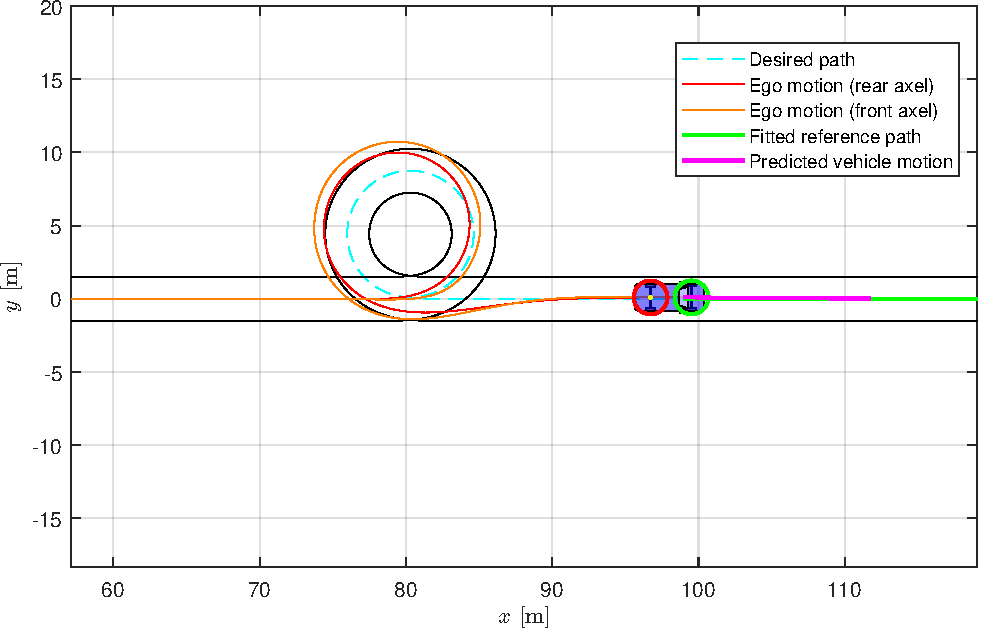
\includegraphics[width=0.5\textwidth]{figures/3_Implementierung/Curve_negative/test_curve_negative_depiction.pdf}
    \caption{Darstellung des Szenarios: Kurvenfahrt negativ}
    \label{fig:test_curve_negative_depiction}
\end{figure}

\subsection{Parametrierung}
Die Parameter für dieses Szenario sind:
\begin{itemize}
    \item maximale Querbeschleunigung in der Kurve $[m\cdot s^{-2}]$: $a_{Lat} \in [1,4]$
    \item Kurvenradius $[m]$: $s_{radius} \in [0.7,0.9]\cdot r_{min,turn}$
    \item verwendetes MPC Parameterset
\end{itemize}

\subsection{abgetestete KPIs}
Es wurden Test für folgende KPIs mit den dazugehörigen Grenzwerten implementiert:

\medskip\noindent\textbf{laterale Ablage:} die Abweichung des Fahrzeugs vom gewünschten Pfad muss größer sein als ein definierter Grenzwert: $s_{error,lat} > kpi_{s_{error,lat}}$

\noindent Wie erwartet führen kleinere Kurvenradien zu größeren maximalen Pfadabweichungen, Abbildung \ref{fig:Curve_negative_s-Error}. Nachdem die Kurve durchfahren ist kann dieser Fehler wieder abgebaut werden.
\begin{figure}[ht]
    \centering
    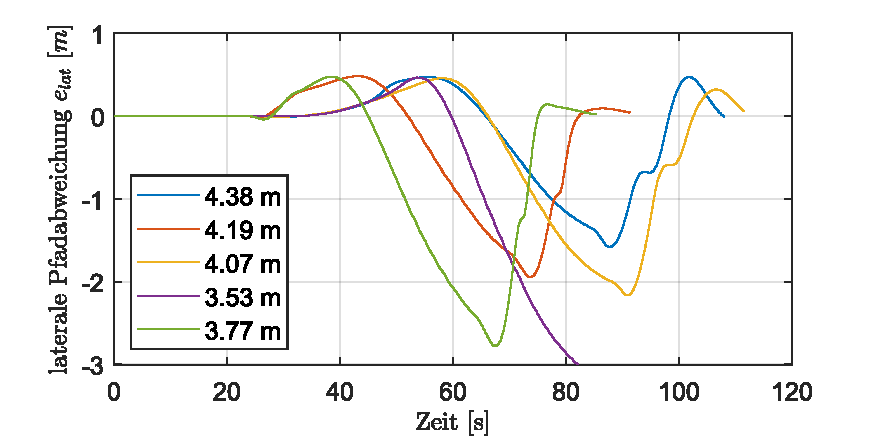
\includegraphics[width=0.5\textwidth]{figures/3_Implementierung/Curve_negative/Curve_negative_s-Error.pdf}
    \caption{KPI Pfadabweichung bei verschiedenen Kurvenradien}
    \label{fig:Curve_negative_s-Error}
\end{figure}

\section{Szenario: ACC mit konstanter Objektgeschwindigkeit} \label{sec:acc_vel_const}
Das Ego startet mit einer Initialgeschwindigkeit auf einer Geraden. Ein Target fährt vor dem Ego mit konstanter Geschwindigkeit. Es exisitiert eine Geschwindigkeitsdifferenz zwischen Ego und Target. Ebenfalls kann die initiale Zeitlücke abweichend von der gewünschten Zeitlücke sein. Das Ego sollte die Geschwindigkeitsdifferenz beseitigen und die gewünschte Zeitlücke herstellen.
\begin{figure}[ht]
    \centering
    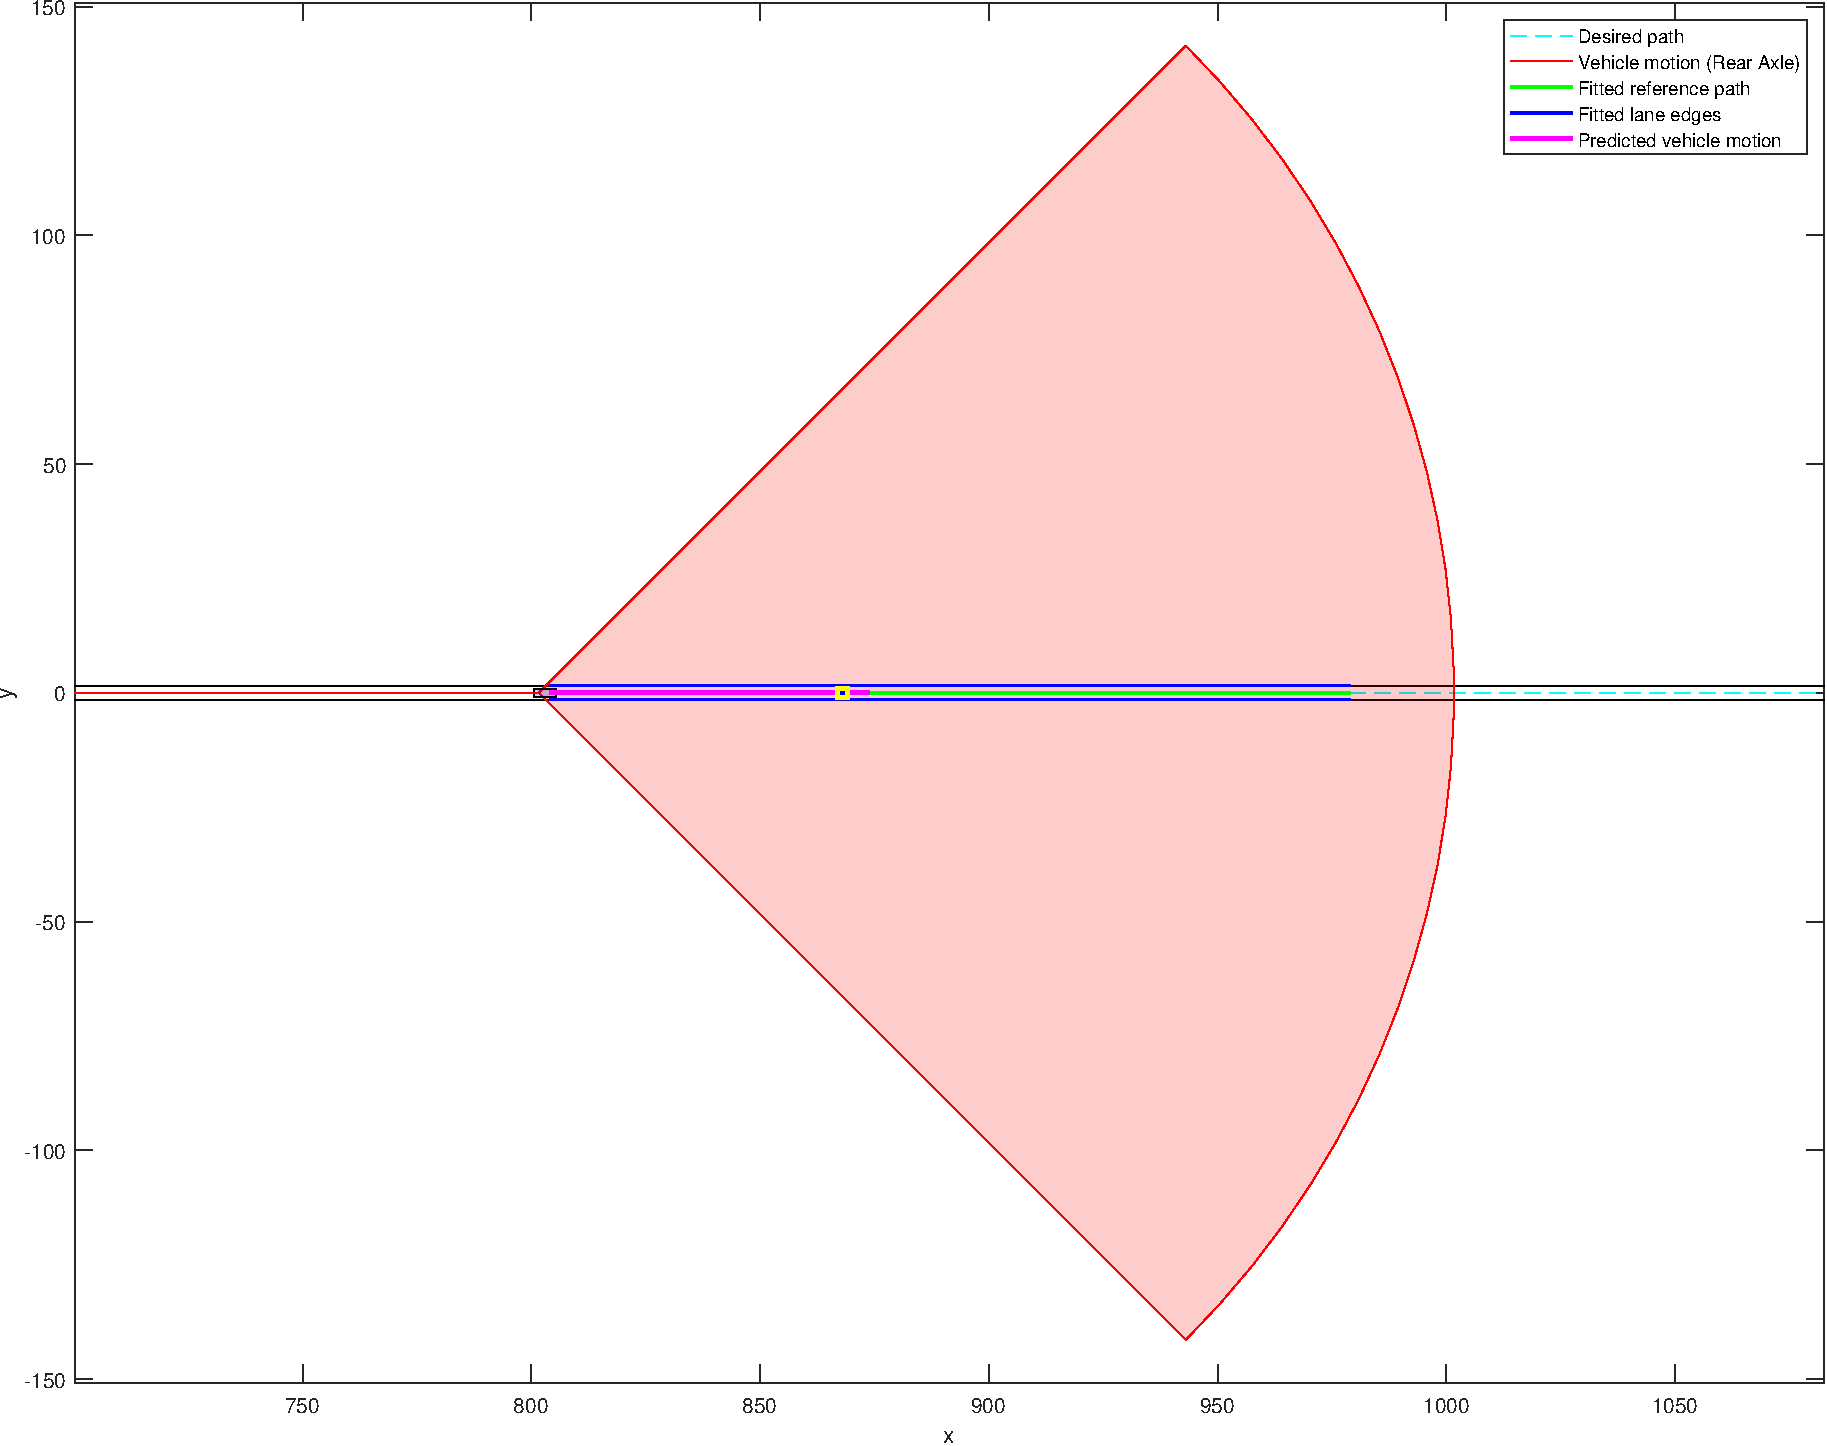
\includegraphics[width=0.5\textwidth]{figures/3_Implementierung/ACC_Vel_Const/test_ACC_Vel_Const_depiction.pdf}
    \caption{Darstellung des Szenarios: ACC mit konstanter Objektgeschwindigkeit}
    \label{fig:test_ACC_Vel_Const_depiction}
\end{figure}

\subsection{Parametrierung}
Die Parameter für dieses Szenario sind:
\begin{itemize}
    \item Initialgeschwindigkeit $[km\cdot h^{-1}]$: $v_{Ego} \in [0.2\cdot v_{vehicle,max}, 0.8\cdot v_{vehicle,max}]$
    \item Differenzgeschwindigkeit $[km\cdot h^{-1}]$: $v_{diff} \in [-0.2,0.2]\cdot v_{Ego}$
    \item Zeitlückenabweichung $[s]$: $t_{offset} \in [-1,1] + t_{gap,desired}$
    \item verwendetes MPC Parameterset
\end{itemize}

\subsection{Abgetestete KPIs}
Es wurden Test für folgende KPIs mit den dazugehörigen Grenzwerten implementiert:

\medskip\noindent\textbf{longitudinale Beschleunigung:} der Gleitende Mittelwert über eine halbe Sekunde darf einen definierten Grenzwert nicht überschreiten: $a_{Long} < kpi_{a_{Long}}$

\medskip\noindent\textbf{longitudinaler Ruck:} der Gleitende Mittelwert über eine halbe Sekunde darf den Grenzwert nicht überschreiten: $j_{Long} < kpi_{j_{Long}}$

\noindent Auftretende longitudinale Rücke und Beschleunigungen sind stark abhängig von der gewählten Paramtrierung. Eine Verletzung der Grenzwerte ist hier nicht zulässig. Vorallem darf die maximale Beschleunigung nicht größer sein als ein definierter Grenzwert. Sowohl Beschleunigung als auch Ruck befinden sich in einem akzeptablem Rahmen, siehe Abbildung \ref{fig:ACC_KPI_a_j}.

\begin{figure}[ht]
    \centering
    \begin{subfigure}[b]{.49\textwidth}
        \centering
        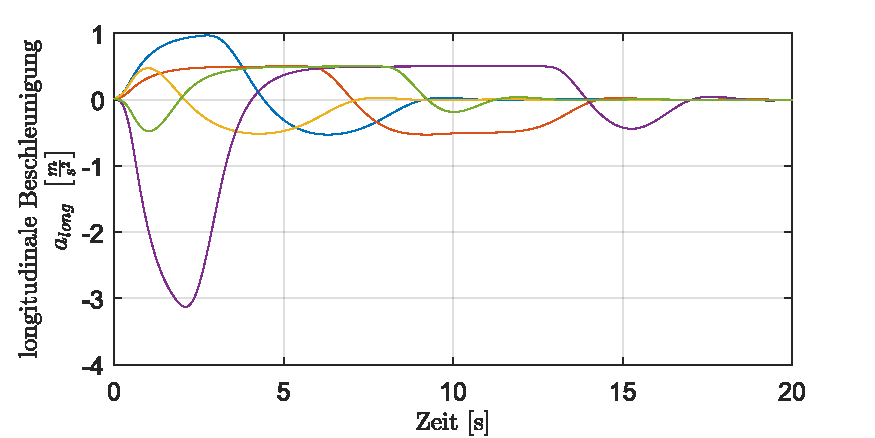
\includegraphics[width=\textwidth]{figures/3_Implementierung/ACC_Vel_Const/ACC_Vel_Const_a-Long.pdf}
    \end{subfigure}
    \hfill
    \begin{subfigure}[b]{.49\textwidth}
        \centering
        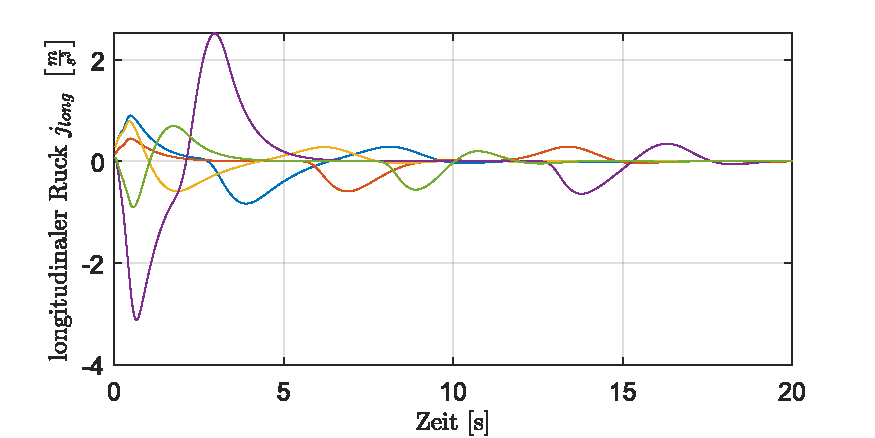
\includegraphics[width=\textwidth]{figures/3_Implementierung/ACC_Vel_Const/ACC_Vel_Const_j-Long.pdf}
    \end{subfigure}
    \caption{Simulationsdaten für Abstands- und Distanzfehler bei unterschiedlichen Parametrierungen}
    \label{fig:ACC_KPI_a_j}
\end{figure}

\medskip\noindent\textbf{Einschwingzeit:} der gewünschte Abstand zum Target sollte innerhalb einer definierten Zeit eingestellt werden: $t_{settle} < kpi_{t_{settle}}$

\noindent Durch ein optimales Systemverhalten kann die Einschwingzeit deutlich veringert werden. Allerdings ist die Definition eines festen Grenzwertes nicht möglich, da diese stark Parametrierungsabhängig ist (Abbildung \ref{fig:ACC_KPI_s_v}). 

\medskip\noindent\textbf{Reaktionszeit:} der Minimalabstand zum Target soll innerhalb einer definierten Zeit hergestellt werden: $t_{reaction} < kpi_{t_{reaction}}$

\noindent Das schnelle einstellen des Mindestabstandes ist wichtiger als die korrekte Abstandseinstellung, weswegen hier ein kürzeres Zeitfenster gewählt wurde.
\begin{figure}
    \centering
    \begin{subfigure}[b]{.49\textwidth}
        \centering
        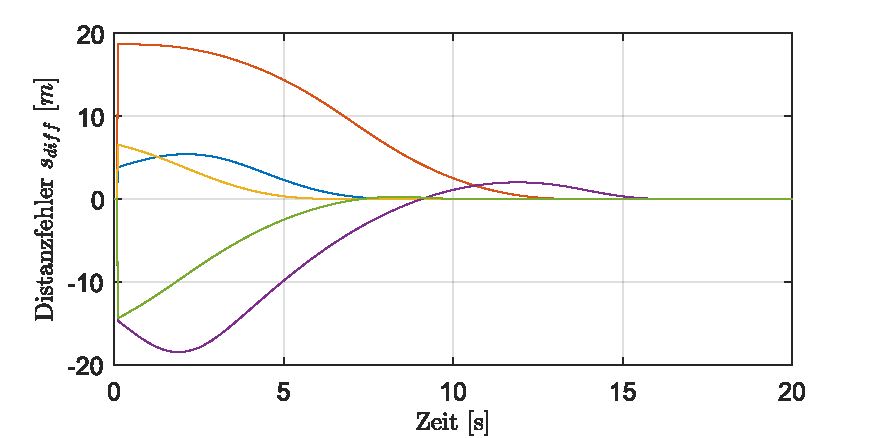
\includegraphics[width=\textwidth]{figures/3_Implementierung/ACC_Vel_Const/ACC_Vel_Const_s-Diff.pdf}
    \end{subfigure}
    \hfill
    \begin{subfigure}[b]{.49\textwidth}
        \centering
        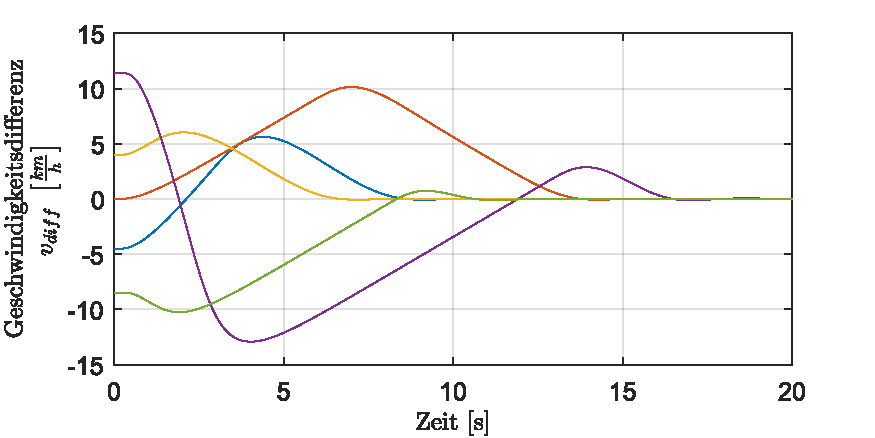
\includegraphics[width=\textwidth]{figures/3_Implementierung/ACC_Vel_Const/ACC_Vel_Const_v-Diff.pdf}
    \end{subfigure}
    \caption{Simulationsdaten für longitudinale Beschleunigung und Ruck bei unterschiedlichen Parametrierungen}
    \label{fig:ACC_KPI_s_v}
\end{figure}